\documentclass[aspectratio=169, professionalfonts]{beamer}

\usetheme{Szeged}
\usecolortheme{dolphin}

\usepackage{amsmath, amssymb, bm}
\usepackage{tikz}
\usetikzlibrary{positioning, arrows.meta, decorations.pathreplacing, calc}
\usepackage{pgfplots}
\pgfplotsset{compat=1.18}

\def\R{\mathbb{R}}
\def\E{\mathbb{E}}
\def\Var{\text{Var}}
\def\Bias{\text{Bias}}
\def\MSE{\text{MSE}}

\definecolor{mantis}{RGB}{0, 105, 62}

\setbeamercolor{frametitle}{fg=white, bg=mantis}
\setbeamercolor{title}{fg=white, bg=mantis}
\setbeamercolor{structure}{fg=mantis}
\setbeamercolor{block title}{bg=mantis, fg=white}
\setbeamercolor{block body}{bg=mantis!10}

\title{Linear Regression}
\subtitle{From Least Squares to Regularisation}
\author{Lebnet Tech Fellows Program}
\date{}

\begin{document}

% ------------------------------------------------------------------
\begin{frame}
\titlepage
\end{frame}

% ------------------------------------------------------------------
\begin{frame}{Roadmap}
\tableofcontents
\end{frame}

% ==================================================================
\section{The Problem}
% ==================================================================

% ------------------------------------------------------------------
\begin{frame}{What Is Linear Regression?}

Given an explanatory variable $x$ and a response $y$, assume:
$$Y = a + bX + \varepsilon$$

where $\varepsilon$ captures noise we do not fully understand.

\bigskip

\textbf{Goal:} find estimators $\hat{a}, \hat{b}$ of the true parameters.

\bigskip

\begin{itemize}
  \item $x \in \R$: univariate regression
  \item $x \in \R^d$: multivariate regression
\end{itemize}

\end{frame}

% ------------------------------------------------------------------
\begin{frame}{Running Example: Ohm's Law}

\begin{columns}[c]
\column{0.45\textwidth}
Voltage and current: $V = IR$.

\begin{itemize}
  \item Measurements $(I_i, V_i)$ from a circuit
  \item Fit a line to estimate resistance $R$
  \item $I$ is explanatory, $V$ is response
\end{itemize}

\column{0.55\textwidth}
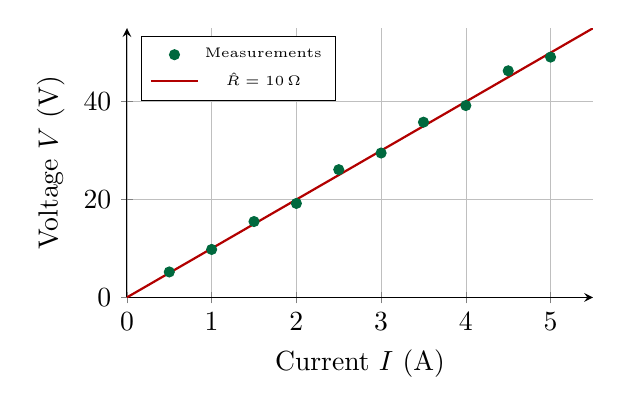
\begin{tikzpicture}
\begin{axis}[
    width=7.5cm, height=5cm,
    xlabel={Current $I$ (A)},
    ylabel={Voltage $V$ (V)},
    xmin=0, xmax=5.5, ymin=0, ymax=55,
    grid=both,
    grid style={line width=.1pt, draw=gray!30},
    major grid style={line width=.2pt, draw=gray!50},
    axis lines=left,
    legend style={font=\tiny, at={(0.03,0.97)}, anchor=north west},
]
\addplot[only marks, mark=*, mark size=1.8pt, color=mantis]
  coordinates {(0.5,5.2)(1,9.8)(1.5,15.5)(2,19.2)(2.5,26.1)
               (3,29.5)(3.5,35.8)(4,39.2)(4.5,46.3)(5,49.1)};
\addplot[domain=0:5.5, samples=2, color=red!70!black, thick] {10*x};
\legend{Measurements, $\hat{R}=10\,\Omega$}
\end{axis}
\end{tikzpicture}
\end{columns}

\end{frame}

% ==================================================================
\section{Why Squared Loss?}
% ==================================================================

% ------------------------------------------------------------------
\begin{frame}{Measuring the Error}

For a candidate line $\hat{y} = a + bx$, the \textbf{vertical distance}
from $(x_i, y_i)$ is natural: we are predicting $y$ from $x$.

\bigskip

The \textbf{squared loss}:
$$\ell(y, \hat{y}) = (y - \hat{y})^2$$

\bigskip

\textbf{Empirical risk} (what we minimise):
$$\hat{\mathcal{R}}_n(f)
  = \frac{1}{n}\sum_{i=1}^{n}(y_i - f(x_i))^2$$

\end{frame}

% ------------------------------------------------------------------
\begin{frame}{Bayes Optimality of Squared Loss}

Under squared loss, the \textbf{Bayes optimal predictor} is the
conditional expectation:
$$f_*(x) = \E[Y \mid X = x]$$

\bigskip

The \textbf{Bayes risk} (irreducible error):
$$\mathcal{R}^* = \E_X\!\bigl[\Var(Y \mid X)\bigr]$$

\bigskip

Linear regression approximates $\E[Y \mid X]$ with the best
linear function. If the true conditional expectation is linear,
the model is correctly specified.

\end{frame}

% ==================================================================
\section{The OLS Solution}
% ==================================================================

% ------------------------------------------------------------------
\begin{frame}{Matrix Formulation}

Stack all observations:
$$\mathbf{y} = \mathbf{X}\bm{\theta} + \bm{\varepsilon}$$

\begin{itemize}
  \item $\mathbf{y} \in \R^n$: response vector
  \item $\mathbf{X} \in \R^{n \times d}$: design matrix
        (first column is all ones for the intercept)
  \item $\bm{\theta} \in \R^d$: parameter vector
\end{itemize}

\bigskip

Empirical risk:
$$\hat{\mathcal{R}}_n(\bm{\theta})
  = \frac{1}{n}\|\mathbf{y} - \mathbf{X}\bm{\theta}\|_2^2$$

\end{frame}

% ------------------------------------------------------------------
\begin{frame}{Deriving the OLS Estimator}

Set $\nabla\hat{\mathcal{R}}_n = \mathbf{0}$:

$$\frac{2}{n}\bigl(\mathbf{X}^\top\mathbf{X}\bm{\theta}
  - \mathbf{X}^\top\mathbf{y}\bigr) = \mathbf{0}$$

\bigskip

This gives the \textbf{normal equations}:
$$\mathbf{X}^\top\mathbf{X}\hat{\bm{\theta}}
  = \mathbf{X}^\top\mathbf{y}$$

\bigskip

If $\mathbf{X}$ has full column rank ($\text{rank}(\mathbf{X}) = d$):

$$\boxed{\hat{\bm{\theta}}
  = (\mathbf{X}^\top\mathbf{X})^{-1}\mathbf{X}^\top\mathbf{y}}$$

\end{frame}

% ==================================================================
\section{Geometric Interpretation}
% ==================================================================

% ------------------------------------------------------------------
\begin{frame}{OLS as Orthogonal Projection}

$\mathbf{y}$ typically does not lie in $\text{Im}(\mathbf{X})$.

\bigskip

OLS finds the closest point in that subspace:
$$\hat{\mathbf{y}}
  = \mathbf{X}\hat{\bm{\theta}}
  = \underbrace{\mathbf{X}(\mathbf{X}^\top\mathbf{X})^{-1}\mathbf{X}^\top}_%
    {\mathbf{P}_{\mathbf{X}}}\,\mathbf{y}$$

\bigskip

\begin{itemize}
  \item $\mathbf{P}_{\mathbf{X}}$: projection matrix onto
        $\text{Im}(\mathbf{X})$
  \item Residuals $\hat{\bm{\varepsilon}} = \mathbf{y} - \hat{\mathbf{y}}$
        are \textbf{orthogonal} to every column of $\mathbf{X}$
  \item This is exactly the content of the normal equations:
        $\mathbf{X}^\top\hat{\bm{\varepsilon}} = \mathbf{0}$
\end{itemize}

\end{frame}

% ==================================================================
\section{Statistical Properties}
% ==================================================================

% ------------------------------------------------------------------
\begin{frame}{Classical Assumptions}

\begin{block}{Classical Linear Model}
\begin{enumerate}
  \item \textbf{Linearity:} $\mathbf{y} = \mathbf{X}\bm{\theta} + \bm{\varepsilon}$
  \item \textbf{Fixed design:} $\mathbf{X}$ is non-random
  \item \textbf{Exogeneity:} $\E[\bm{\varepsilon} \mid \mathbf{X}] = \mathbf{0}$
  \item \textbf{Spherical errors:}
        $\Var(\bm{\varepsilon} \mid \mathbf{X}) = \sigma^2\mathbf{I}_n$
  \item \textbf{Full rank:} $\text{rank}(\mathbf{X}) = d < n$
\end{enumerate}
\end{block}

For inference, add:

\quad 6.\ \textbf{Normality:}
$\bm{\varepsilon} \mid \mathbf{X} \sim \mathcal{N}(\mathbf{0}, \sigma^2\mathbf{I}_n)$

\end{frame}

% ------------------------------------------------------------------
\begin{frame}{Unbiasedness and Variance}

Substitute the true model into OLS:
$$\hat{\bm{\theta}}
  = \bm{\theta}
  + (\mathbf{X}^\top\mathbf{X})^{-1}\mathbf{X}^\top\bm{\varepsilon}$$

\bigskip

\begin{block}{Under assumptions 1-4}
\begin{align*}
\E[\hat{\bm{\theta}}] &= \bm{\theta}
  &&\text{(unbiased)} \\[6pt]
\Var(\hat{\bm{\theta}}) &= \sigma^2(\mathbf{X}^\top\mathbf{X})^{-1}
\end{align*}
\end{block}

\end{frame}

% ------------------------------------------------------------------
\begin{frame}{Gauss-Markov: OLS is BLUE}

\begin{alertblock}{Gauss-Markov Theorem (assumptions 1-5)}
Among all \textbf{linear unbiased} estimators
$\tilde{\bm{\theta}} = \mathbf{A}\mathbf{y}$:
$$\Var(\tilde{\theta}_j) \ge \Var(\hat{\theta}_j)
  \quad\text{for all } j$$
\end{alertblock}

\bigskip

\textbf{Key idea:} write $\mathbf{A} = \mathbf{A}_{\text{OLS}} + \mathbf{D}$.
Unbiasedness forces $\mathbf{D}\mathbf{X} = \mathbf{0}$, which makes the
cross terms vanish, leaving $\Var(\tilde{\bm{\theta}})
= \Var(\hat{\bm{\theta}}) + \sigma^2\mathbf{D}\mathbf{D}^\top$.

\bigskip

Under normality, OLS is in fact \textbf{BUE} (best among
\emph{all} unbiased estimators).

\end{frame}

% ==================================================================
\section{Bias-Variance Tradeoff}
% ==================================================================

% ------------------------------------------------------------------
\begin{frame}{MSE = Bias$^2$ + Variance}

$$\MSE(\hat{\theta})
  = \E[(\hat{\theta} - \theta)^2]
  = \Bias(\hat{\theta})^2 + \Var(\hat{\theta})$$

\bigskip

For prediction at a new point $\mathbf{x}_0$:

$$\E[(y_0 - \hat{y}_0)^2]
  = \underbrace{\sigma^2}_{\text{irreducible}}
  + \underbrace{\Bias(\hat{y}_0)^2}_{\text{model error}}
  + \underbrace{\Var(\hat{y}_0)}_{\text{estimation noise}}$$

\end{frame}

% ------------------------------------------------------------------
\begin{frame}{The Tradeoff in Practice}

\begin{center}
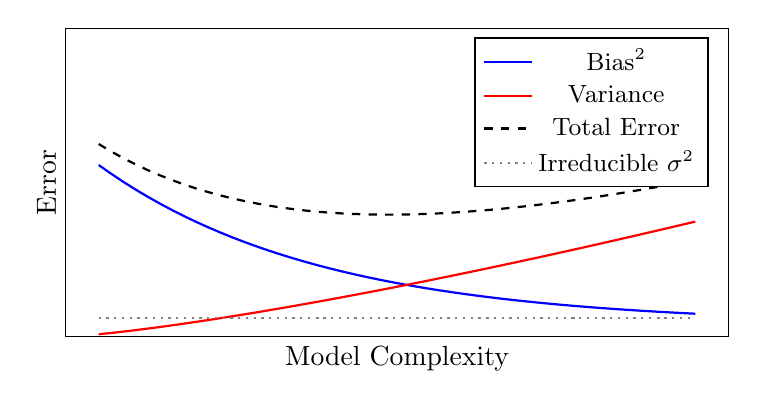
\begin{tikzpicture}
\begin{axis}[
    width=10cm, height=5.5cm,
    xlabel={Model Complexity},
    ylabel={Error},
    xmin=0, xmax=10, ymin=0, ymax=5,
    xtick=\empty, ytick=\empty,
    legend style={font=\small, at={(0.97,0.97)}, anchor=north east},
]
\addplot[domain=0.5:9.5, samples=50, color=blue, thick]
  {3*exp(-0.3*x)+0.2};
\addplot[domain=0.5:9.5, samples=50, color=red, thick]
  {0.1*x^1.3};
\addplot[domain=0.5:9.5, samples=50, color=black, thick, dashed]
  {3*exp(-0.3*x)+0.2+0.1*x^1.3+0.3};
\addplot[domain=0.5:9.5, samples=50, color=gray, dotted, thick]
  {0.3};
\legend{$\text{Bias}^2$, Variance, Total Error, Irreducible $\sigma^2$}
\end{axis}
\end{tikzpicture}
\end{center}

\begin{itemize}
  \item \textbf{Underfitting} (left): high bias, low variance
  \item \textbf{Overfitting} (right): low bias, high variance
  \item \textbf{Sweet spot}: minimise total error
\end{itemize}

\end{frame}

% ==================================================================
\section{Regularisation}
% ==================================================================

% ------------------------------------------------------------------
\begin{frame}{Ridge Regression ($L_2$ Penalty)}

Add a penalty on $\|\bm{\theta}\|_2^2$:

\begin{block}{Ridge Estimator}
$$\hat{\bm{\theta}}_{\text{ridge}}
  = (\mathbf{X}^\top\mathbf{X} + \lambda\mathbf{I})^{-1}
    \mathbf{X}^\top\mathbf{y}$$
\end{block}

\bigskip

\begin{itemize}
  \item \textbf{Biased}, but lower variance than OLS
  \item Always invertible for $\lambda > 0$
        (cures multicollinearity)
  \item Bayesian view: Gaussian prior
        $\bm{\theta}\sim\mathcal{N}(\mathbf{0},\tau^2\mathbf{I})$
        with $\lambda = \sigma^2/\tau^2$
\end{itemize}

\end{frame}

% ------------------------------------------------------------------
\begin{frame}{Lasso ($L_1$ Penalty)}

Replace the $L_2$ penalty with $L_1$:

\begin{block}{Lasso Estimator}
$$\hat{\bm{\theta}}_{\text{lasso}}
  = \arg\min_{\bm{\theta}}\left\{
    \frac{1}{2n}\|\mathbf{y}-\mathbf{X}\bm{\theta}\|_2^2
    + \lambda\|\bm{\theta}\|_1
  \right\}$$
\end{block}

\bigskip

\begin{itemize}
  \item No closed-form solution (solved by coordinate descent)
  \item Produces \textbf{exact zeros}: automatic variable selection
  \item The $L_1$ ball has corners on the axes; the OLS contour
        typically first touches a corner
\end{itemize}

\end{frame}

% ------------------------------------------------------------------
\begin{frame}{Ridge vs Lasso: Geometry}

\begin{columns}[c]
\column{0.5\textwidth}
\centering
\textbf{Ridge ($L_2$)}

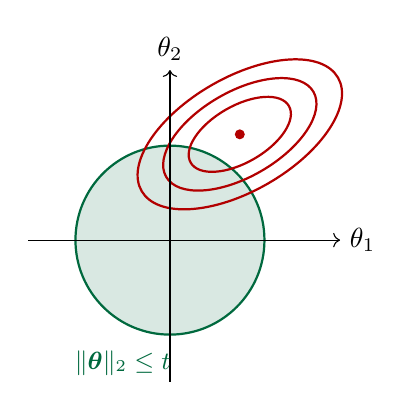
\begin{tikzpicture}[scale=1.2]
\draw[thick, mantis, fill=mantis!15] (0,0) circle (1);
\draw[thick, red!70!black, rotate=30]
  (1.2,0.6) ellipse (0.6 and 0.3);
\draw[thick, red!70!black, rotate=30]
  (1.2,0.6) ellipse (0.9 and 0.45);
\draw[thick, red!70!black, rotate=30]
  (1.2,0.6) ellipse (1.2 and 0.6);
\fill[red!70!black] ({1.2*cos(30)-0.6*sin(30)},
  {1.2*sin(30)+0.6*cos(30)}) circle (1.5pt);
\draw[->] (-1.5,0) -- (1.8,0) node[right] {$\theta_1$};
\draw[->] (0,-1.5) -- (0,1.8) node[above] {$\theta_2$};
\node[mantis, font=\small] at (-0.5,-1.3) {$\|\bm\theta\|_2\le t$};
\end{tikzpicture}

All $\theta_j \neq 0$ (shrinkage)

\column{0.5\textwidth}
\centering
\textbf{Lasso ($L_1$)}

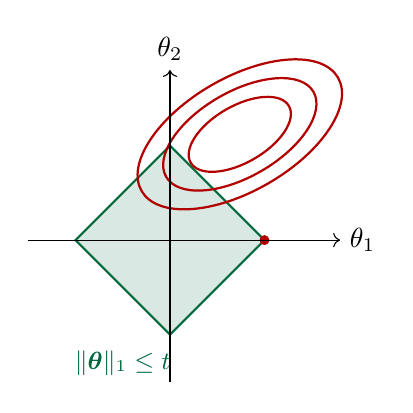
\begin{tikzpicture}[scale=1.2]
\draw[thick, mantis, fill=mantis!15]
  (1,0) -- (0,1) -- (-1,0) -- (0,-1) -- cycle;
\draw[thick, red!70!black, rotate=30]
  (1.2,0.6) ellipse (0.6 and 0.3);
\draw[thick, red!70!black, rotate=30]
  (1.2,0.6) ellipse (0.9 and 0.45);
\draw[thick, red!70!black, rotate=30]
  (1.2,0.6) ellipse (1.2 and 0.6);
\fill[red!70!black] (1,0) circle (1.5pt);
\draw[->] (-1.5,0) -- (1.8,0) node[right] {$\theta_1$};
\draw[->] (0,-1.5) -- (0,1.8) node[above] {$\theta_2$};
\node[mantis, font=\small] at (-0.5,-1.3) {$\|\bm\theta\|_1\le t$};
\end{tikzpicture}

Some $\theta_j = 0$ (sparsity)
\end{columns}

\end{frame}

% ==================================================================
\section{Model Evaluation}
% ==================================================================

% ------------------------------------------------------------------
\begin{frame}{$R^2$: Proportion of Variance Explained}

$$R^2 = 1 - \frac{\text{RSS}}{\text{TSS}}
  = 1 - \frac{\sum(y_i - \hat{y}_i)^2}{\sum(y_i - \bar{y})^2}$$

\bigskip

\begin{itemize}
  \item $R^2 = 1$: perfect fit
  \item $R^2 = 0$: no better than predicting $\bar{y}$
\end{itemize}

\bigskip

\begin{alertblock}{Problem}
$R^2$ \textbf{never decreases} when adding features, even noise.
\end{alertblock}

\textbf{Fix:} Adjusted $R^2$:
$\;\bar{R}^2 = 1 - \dfrac{n-1}{n-d}(1 - R^2)$

\end{frame}

% ------------------------------------------------------------------
\begin{frame}{Cross-Validation}

$k$-fold CV estimates out-of-sample error:

\begin{enumerate}
  \item Split data into $k$ folds
  \item For each fold $i$: train on all folds except $i$,
        evaluate on fold $i$
  \item Average:
        $\;\text{CV}_k = \frac{1}{k}\sum_{i=1}^k \text{MSE}_i$
\end{enumerate}

\bigskip

\begin{itemize}
  \item $k = n$ (leave-one-out): low bias, high variance
  \item $k = 5$ or $10$: good bias-variance balance in practice
  \item Use CV to choose $\lambda$ in Ridge / Lasso
\end{itemize}

\end{frame}

% ==================================================================
\section{Summary}
% ==================================================================

% ------------------------------------------------------------------
\begin{frame}{Recap: The Full Story}

\begin{enumerate}
  \item \textbf{Problem:} predict a continuous $y$ from features $\mathbf{x}$.
  \item \textbf{Loss:} squared error; Bayes optimal predictor is
        $\E[Y\mid X]$.
  \item \textbf{OLS:}
        $\hat{\bm{\theta}} = (\mathbf{X}^\top\mathbf{X})^{-1}
         \mathbf{X}^\top\mathbf{y}$
        (projection onto column space).
  \item \textbf{Properties:} unbiased, BLUE (Gauss-Markov).
  \item \textbf{Tradeoff:} MSE = Bias$^2$ + Variance; complexity
        must be balanced.
  \item \textbf{Regularisation:} Ridge (shrinkage), Lasso (sparsity).
  \item \textbf{Evaluation:} adjusted $R^2$, cross-validation.
\end{enumerate}

\end{frame}

% ------------------------------------------------------------------
{
\setbeamercolor{background canvas}{bg=mantis}
\setbeamercolor{normal text}{fg=white}
\usebeamercolor[fg]{normal text}
\begin{frame}[c]
\centering
\Huge\textbf{Questions?}
\end{frame}
}

\end{document}
